% AEJ-Article.tex for AEA last revised 22 June 2011
\documentclass[AEJ]{AEA}

%%%%%% NOTE FROM OVERLEAF: The mathtime package is no longer publicly available nor distributed. We recommend using a different font package e.g. mathptmx if you'd like to use a Times font.
% \usepackage{mathptmx}

% The mathtime package uses a Times font instead of Computer Modern.
% Uncomment the line below if you wish to use the mathtime package:
%\usepackage[cmbold]{mathtime}
% Note that miktex, by default, configures the mathtime package to use commercial fonts
% which you may not have. If you would like to use mathtime but you are seeing error
% messages about missing fonts (mtex.pfb, mtsy.pfb, or rmtmi.pfb) then please see
% the technical support document at http://www.aeaweb.org/templates/technical_support.pdf
% for instructions on fixing this problem.

% Note: you may use either harvard or natbib (but not both) to provide a wider
% variety of citation commands than latex supports natively. See below.

% Uncomment the next line to use the natbib package with bibtex 
\usepackage{natbib}
\usepackage{hyperref}
\usepackage{acronym}
\usepackage[names]{xcolor}
\usepackage{graphicx}
% Uncomment the next line to use the harvard package with bibtex
%\usepackage[abbr]{harvard}

%%%
%%% TESTING
%%%
\usepackage{blindtext}

\usepackage[most]{tcolorbox}
\usetikzlibrary{calc}

% This command determines the leading (vertical space between lines) in draft mode
% with 1.5 corresponding to "double" spacing.
\draftSpacing{1.5}

%% Acronyms
\acrodef{AEA}{American Economic Association}
\acrodef{DOI}{Digital Object Identifier}
\acrodef{FAIR}{Findable, Accessible, Interoperable, Re-usable}
\acrodef{PSID}{Panel Study of Income Dynamics}
\acrodef{HRS}{Health and Retirement Study}

% reset colors
\definecolor{darkblue}{rgb}{0 0 255}
\hypersetup{colorlinks,breaklinks,citecolor=darkblue,linkcolor=darkblue,urlcolor=darkblue}
\begin{document}
%%% TESTING
\tcbset{
  toplength/.store in={\tcbcornerruletoplength},
  leftlength/.store in={\tcbcornerruleleftlength},
  toplength=3cm,
  leftlength=2cm,
  bottomlength/.store in={\tcbcornerrulebottomlength},
  rightlength/.store in={\tcbcornerrulerightlength},
  bottomlength=3cm,
  rightlength=2cm,
  cornerruleshift/.store in={\tcbcornerruleshift},
  cornerruleshift=1pt,
  topcornercolor/.store in={\tcbtopcornercolor},
  bottomcornercolor/.store in={\tcbbottomcornercolor},
  topcornercolor=green!40!blue,
  bottomcornercolor=blue!40!green,
}

\newtcolorbox{cornerbox}[1][]{%
  enhanced jigsaw,
  sharp corners,
  boxrule=0pt,
  underlay={
    \coordinate (topend) at ($(frame.north west) + (0:\tcbcornerruletoplength)$);
    \coordinate (leftend) at ($(frame.north west) - (90:\tcbcornerruleleftlength)$);
    \coordinate (bottomend) at ($(frame.south east) - (0:\tcbcornerrulebottomlength)$);
    \coordinate (rightend) at ($(frame.south east) + (90:\tcbcornerrulerightlength)$);
    \draw[line width=2pt,\tcbtopcornercolor] ([xshift=-\tcbcornerruleshift]leftend) -- ([shift={(-\tcbcornerruleshift,\tcbcornerruleshift)}]frame.north west) -- ([shift={(-\tcbcornerruleshift,\tcbcornerruleshift)}] topend);
    \draw[line width=2pt,\tcbbottomcornercolor] ([xshift=\tcbcornerruleshift]rightend) -- ([shift={(\tcbcornerruleshift,-\tcbcornerruleshift)}]frame.south east) -- ([shift={(-\tcbcornerruleshift,-\tcbcornerruleshift)}] bottomend);
  },
  #1,
}


%%% END TESTING
\title{Report for 2018 by the AEA Data Editor }
\shortTitle{Report by Data Editor}
\author{Lars Vilhuber\thanks{%
Vilhuber: Cornell University, lars.vilhuber@cornell.edu.}}
\date{\today}
\pubMonth{Month}
\pubYear{Year}
\pubVolume{Vol}
\pubIssue{Issue}
\JEL{}
\Keywords{}

\begin{abstract}
Your abstract here.
\end{abstract}

\maketitle
The purpose of scientific publishing is the dissemination of robust research findings, exposing them to the scrutiny of peers. Key to this endeavor is documenting the provenance of those findings. For empirical articles, the foundations on which they reside are external to the article, and often to the journal, in which they are published. Our scientific community faces  increasingly complex issues of privacy and confidentiality that prevent ``open'' access to those same sources. In consequence, there is a need to properly cite the digital inputs to our published output and to properly curate those inputs.  

Many scientists,  journals, learned societies, and funding agencies have called for greater transparency of research practices, and more assurance that published research is reproducible \citep{Stodden2016-uc,Fuentes2016-wz,Moffitt2016-wl,Camerer2016-kl,Bollen2015-vb,Joskow2015-hd}. This has lead to a focus on transparent access to research data and code \citep{Coffman2017-si,Hoeffler2017-aa,Duvendack2017-js,Hamermesh2017-kq}. This interim report describes the current conceptual and practical issues, outlines the \ac{AEA}'s efforts, through the new position of Data Editor,  to address these issues, and highlights some of the short- and medium-term changes that economists might expect. 


\section{The current environment}

The \ac{AEA}'s data and code posting policy \citep{American_Economic_Association2008-az}, as well as that of other societies and journals, are intended to create a minimal framework from which to replicate empirical findings. Many partial solutions have been implemented. A few journals have implemented verification of submitted code and data during the editorial process,%
\footnote{The American Journal of Political Science outsources this activity to the Odum Institute for Research in Social Science (CITE). The Journal of the American Statistical Association performs a "broad evaluation of quality and potential for usability of the code and data" since 2016 \citep{Stodden2016-uc}.}
highlight the verification on data archives \citep{Open_Science_Framework2017-zc}, maintain lists of acceptable third-party repositories,%
\footnote{Nature Scientific Data maintains a list for its journals \citep{Nature_Scientific_Data2016-hl}, and other institutions (CoreTrustSeal, FAIRsharing) have as their primary purpose to perform this kind of vetting.} 
and interlink with collaborating repositories to highlight authors' (and repositories') contributions to the data component of a scholarly work.%
\footnote{Elsevier interlinks, for instance, with ICPSR, highlighting the use of a repository on the article's web page.}
Outside of journals, several projects are working to educate the community to incorporate principles of replicability and traceability into their workflow.%
\footnote{Open Science Framework, Project TIER, BITSS are just a few of those active in that field \citep{Gentzkow2014-va,Wilson2016-bt}.}
No journal currently does, in my opinion, an adequate job of providing information about restricted-access data, in part because most restricted-access data centers cannot provide structured information about existence, modalities of access, or even data landing pages.%
\footnote{Restricted-access data hosted on ICPSR and possibly Harvard Dataverse are notable exceptions. On the journal side, Elsevier journals have experimented with "Data Descriptions", but while the form is machine-readable, it is essentially free-form text, and checking the box "confidential data" essentially stops the process of filling in any information.} 
None of these solutions are widespread, and standards are only now being developed.

\begin{cornerbox}
In the summer of 2018, I had the privilege of contributing a white paper to the Committee on Reproducibility and Replicability in Science of the National Academies of Science on the history and state of reproducibility in economics. In many sciences, new preprint services have emerged within the last two years, e.g., \href{https://psyarxiv.com/}{PsyArXiv}. These are considered to be part of the broader move to greater research transparency. While writing the white paper, I pointed out that this kind of pre-publication exchange has long been the norm in economics. The first National Bureau of Economic Research (NBER) working paper, one of the most prestigious working paper series in economics, was published (in paper form) in 1973 \citep{WelchEducationInformationEfficiency1973}. By the early 1990s, there was a wide variety of such working paper series, typically provided by academic departments and research institutions. Since grey literature at the time was not cataloged or indexed by most bibliographic indexes, a distinct effort to identify both working papers and the novel electronic versions grew from modest beginnings in 1992 at Université de Montréal and elsewhere into what is today known as the Research Papers in Economics (RePEc) network, a “collaborative effort by hundreds of volunteers in 99 countries” \citep{RePEcResearchPapers,KrichelEconomicsOpenBibliographic2009,Batiz-Lazobriefbusinesshistory2012}. The initial index was split into electronic (WoPEc) \citep{KrichelWoPEcElectronicWorking1997}  and printed working papers (BibEc) \citep{KrichelEconomicsOpenBibliographic2009,CruzCatalogingEconomicsPreprints2000}, testimony to the prevalence of the exchange of scientific research in semi-organized ways.  In 1997, BibEc counted 34,000 working papers from 368 working paper series (30). RePEc today has data from around 4,600 working paper series and claims about 2.5 million full-text (free) research items, provided in a decentralized fashion by about 2,000 archives (31). These items not only include traditional research papers, but also, since 1994, computer code (32–34). 
\end{cornerbox}

\section{Definitions}
A brief definition of the terms ``replicable'' and ``reproducible'' is in order. The terms are somewhat ambiguously defined in the scientific community. We will use the definitions used by \cite{Bollen2015-vb}. ``Reproducibility''  refers to the ability of researchers to achieve the same results as previous researchers, using the same data and same analysis methods, and ``replicability''  refers to the ability of researchers, using the same analysis methods, to duplicate results using ``new'' data. Other authors may use similar or conflicting terms \citep{Clemens2017-zj}. 

\section{Implementing improved transparency of research}
A modern data and code availability policy should support both reproducibility and replicability, by supporting accurate and transparent description of the provenance of the scientific results. In particular, a functional implementation of those concepts suggests that both data and code need to be subject to the \ac{FAIR} principles \cite{FORCE11FAIRDATAPRINCIPLES}: findable, accessible, interoperable, and re-usable. In this context, we interpret the ``interoperability'' of code as ``code that works, and the workings of which are comprehensible by a third party'' (CITE??). 

\subsection{Goal 1: Improved findability of data used in research articles}

Under this goal, we start by abolishing journal-specific ``supplementary materials'' as the primary repository of data and code that are part of the provenance chain of an article. As currently implemented at most journals, including the \ac{AEA}'s journals, they lack findability, proper citability as first-class objects, and are somewhat opaque (packaged as ZIP files). Historical materials will be migrated to a new curated archive at ICPSR. The AEA's ``Data and Code Archive @ ICPSR'' will display the full contents of the materials as deposited by authors in the past, without the need to download ZIP files. The materials will receive their own citable \ac{DOI}. Through the \ac{DOI} registrars, we automatically leverage the ability to link and associate the archives with their original articles. 

On the AEA's journal websites, the links to ``supplementary'' materials will initially appear to be the same (although pointing to the new locations), but future enhancements will allow for greater visibility or transparency of the associated materials. However, by separating the hosting of data archives (for historical materials, at ICPSR) from the referencing of those archives, we open the door to a more consistent model of linking to and citing data artifacts associated with published articles.

For future submissions, we will allow researchers to reference supplementary materials on a wide list of data archives or repositories.\footnote{Do I need to distinguish the two? is there a difference?} 
In particular, while some journals are already curating a list of recommended \textit{open} data archives \citep{Nature_Scientific_Data2016-hl} (ALSO PLOS, F1000), we will also allow authors to reference materials in reliable \textit{restricted-access} data repositories. What constitutes a ``reliable'' data repository? For one, it needs \textit{persistence}, and \textit{accessibility}. Properly managed repositories have a \textit{preservation policy} - they commit to maintaining deposits for a defined duration (often, but not always, in perpetuity), and only under very restrictive circumstances will remove deposits. Such repositories will also have a policy about access - who can obtain data deposited at the institution, and under what conditions. This characterization applies homogeneously to open and restricted-access repositories. A recommended repository will have been vetted (by the AEA Data Editor, or a reliable third party) to have acceptable and credible policies. 

Authors submitting their work to the AEA journals will be affected in several ways. First, those authors who already deposit their (open access) code and data at known repositories will not have to do so again - a simple reference (and citation!) of the previously archived materials is sufficient. Authors who use data provided through institutional providers (\ac{PSID}, \ac{HRS}, the U.S. Census Bureau, and international equivalents), and who in some cases cannot deposit the data, will also reference the persistent location where they obtained their data from, and where others can do so as well. In the case of restricted-access, a better description of access procedures will be requested from authors, who in turn should ask their data providers to provide such procedural descriptions, in the form of web pages and (persistent and citable) documents. 



If replicability is truly part of the research scientist's workflow, then by the time she submits an article to any journal, the intermediate and final data products as well as the code used for an article have already been deposited at appropriate repositories and archives. If all such repositories and archives are of sufficient quality, then the additional deposit at a journal is duplicative at best, and perturbative to the provenance chain at worst. The right solution is to reference those other repositories, not copy them. Of course, for those that have not used repositories and simply wish to provide a replication zip archive of the files on their laptop, an adequate deposit solution should also exist.
By fundamentally relying on references to repositories instead of deposits, it also becomes possible to put public-use and restricted-access data on a comparable footing at the journal with regards to potential replicability. Well documented location of data (through DOI), access protocols (implicit or click-through license, contracts, etc.), and access mechanism (direct download, delivery of physical media or controlled download, sign-on to controlled secure access, etc.) are then available for any data.

\section{Goal 2: Improved Reliability of Replication Materials}
\begin{figure}
    \centering
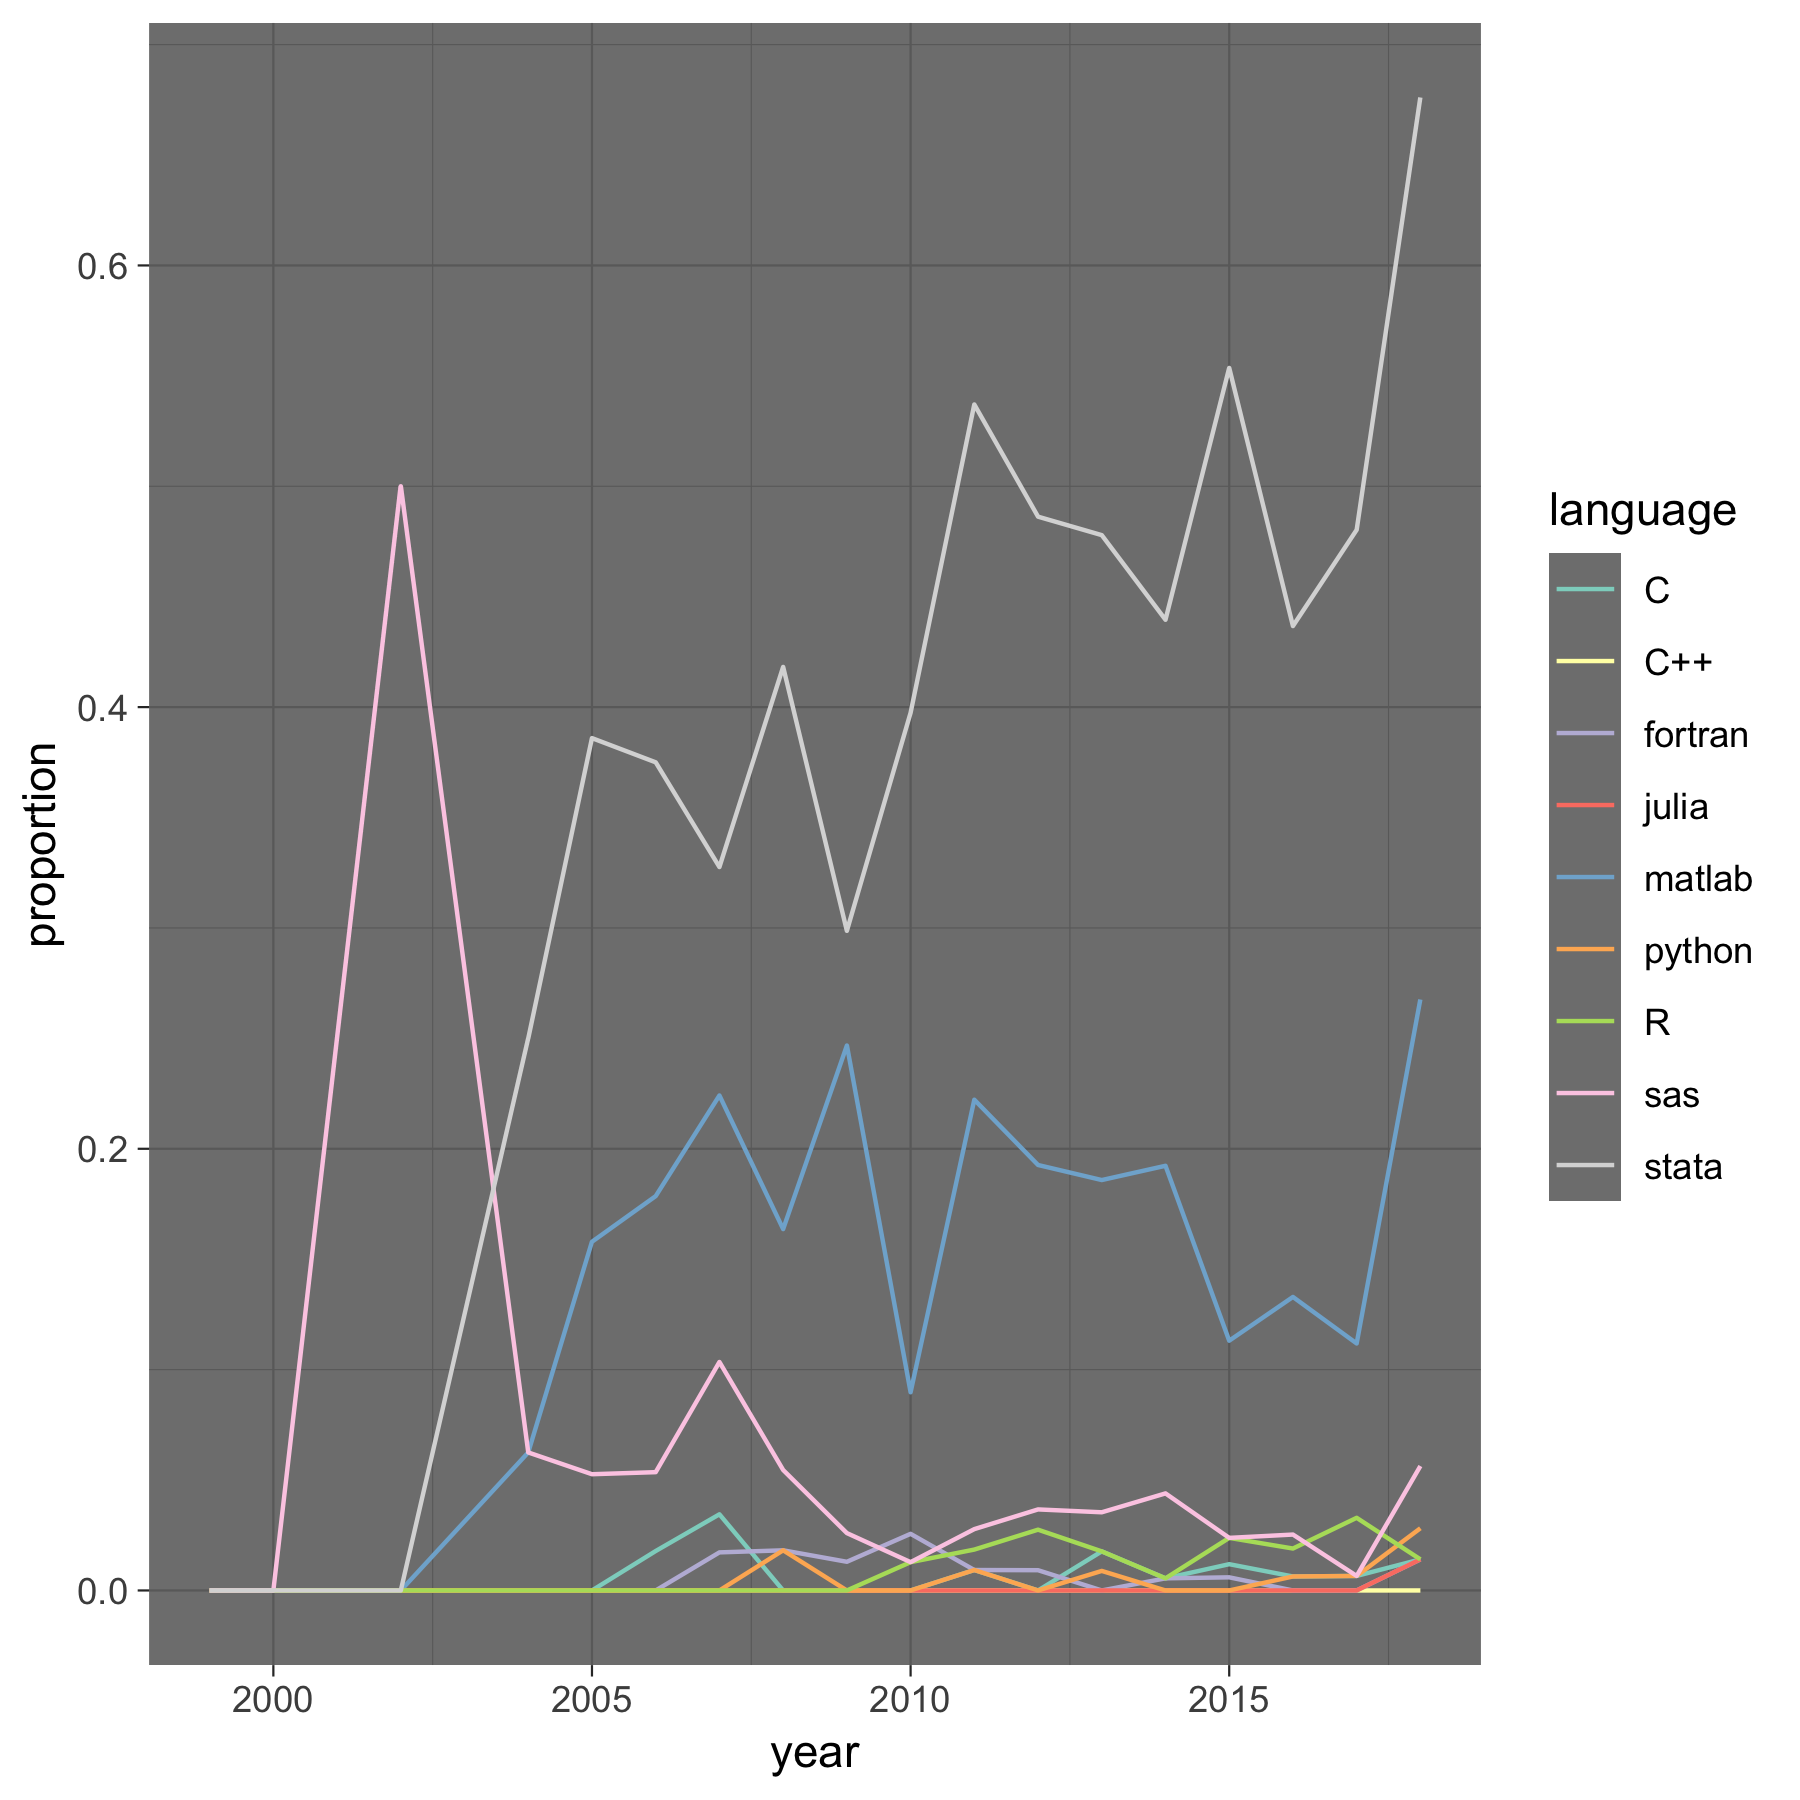
\includegraphics[width=0.7\textwidth]{images/aer_programs_by_year.png}
    \caption{Popularity of statistical software in the AER}
    \label{fig:aer_programs_by_year}
    \footnotesize Figure provided by Patrick Baylis (UBC), based on filename extensions in ZIP files of replication materials on the AEA website.
\end{figure}

\section{Data Citations}
Properly referencing data goes beyond just reproducibility - it is also proper scientific writing style. In the same way that we use bibliographic references to ``printed'' resources, we should also be using such references for data resources, to give and receive credit where credit is due. Not referencing an article or book is at best an oversight, and at worst plagiarism - and the same should apply to data objects. Numerous guides and tutorials exist  \citep{dataone-l09,icpsr-data-cite,force11declaration}.

The AEA uses the Chicago style for citations and bibliographies \citep{aeadatarefs}. However, the Chicago Style Manual \citep{citation-machine,ChicagoManualofStyleChicagoManualStyle2018} does not provide examples for data citations, and neither does the Citation Style Language\footnote{\url{https://citationstyles.org/}} used by applications like Zotero\footnote{\url{https://www.zotero.org/}} and Mendeley Desktop\footnote{\url{https://www.mendeley.com/download-desktop/}}.


As part of our activities, the AEA prepress department has started the process of updating AEA templates available through such software.\footnote{For the technically inclined, this process involves updating an existing style or creating a new style on \url{https://citationstyles.org/} and \url{https://github.com/citation-style-language/styles}, from where it propagates to a large number of software packages.} Some guidance for data citations is provided at 


% Remove or comment out the next two lines if you are not using bibtex.
\bibliographystyle{aea}
\bibliography{paper,references,zotero}

% The appendix command is issued once, prior to all appendices, if any.
\appendix

\section{Reviewers}

\end{document}

